\chapter{\IfLanguageName{dutch}{Data exploration}{Data exploration}}
\label{ch:dataexploration}

Before building any predictive models, we first perform exploratory data analysis (EDA) to understand the structure, trends, and relationships within the dataset.
This step helps uncover patterns, detect anomalies or missing values, and identify correlations between variables.
In this section, we examine the historical price behavior of Bitcoin and Tezos, assess their correlation, and explore key metrics such as returns, trading volume, and market capitalization.

\subsection{Bitcoin and Tezos Price History}
\label{sec:pricehistory}

\subsubsection{Price History of Bitcoin}
\label{sec:btc-pricehistory}
\begin{figure}[H]
    \centering
    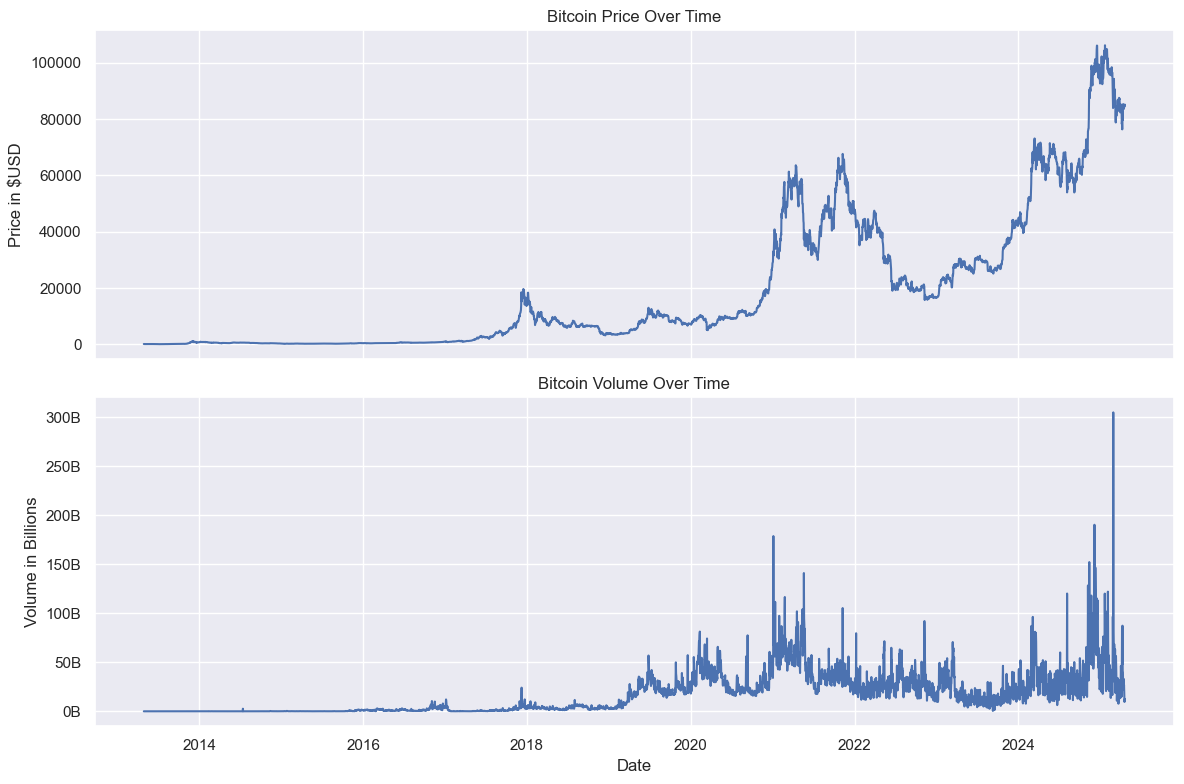
\includegraphics[width=0.8\textwidth]{Bitcoin_price_volume.png}
    \caption{Daily Bitcoin trading volume over time.}
    \label{fig:btc-volume}
\end{figure}

The figure illustrates the daily trading volume and price of Bitcoin over time.
 A notable simultaneous peak in both price and volume occurred at the end of 2024, with Bitcoin reaching an all-time high of \$109,114.88 and recording a daily trading volume exceeding \$300 billion. Additionally, the chart reveals data limitations in the earlier years, particularly between 2013 and 2014, where trading volume data is absent.
 These omissions, attributed to historical data availability issues, were addressed in Section~\ref{ch:datacollection}.

\subsubsection{Price History of Tezos}
\label{sec:xtz-pricehistory}
\begin{figure}[H]
    \centering
    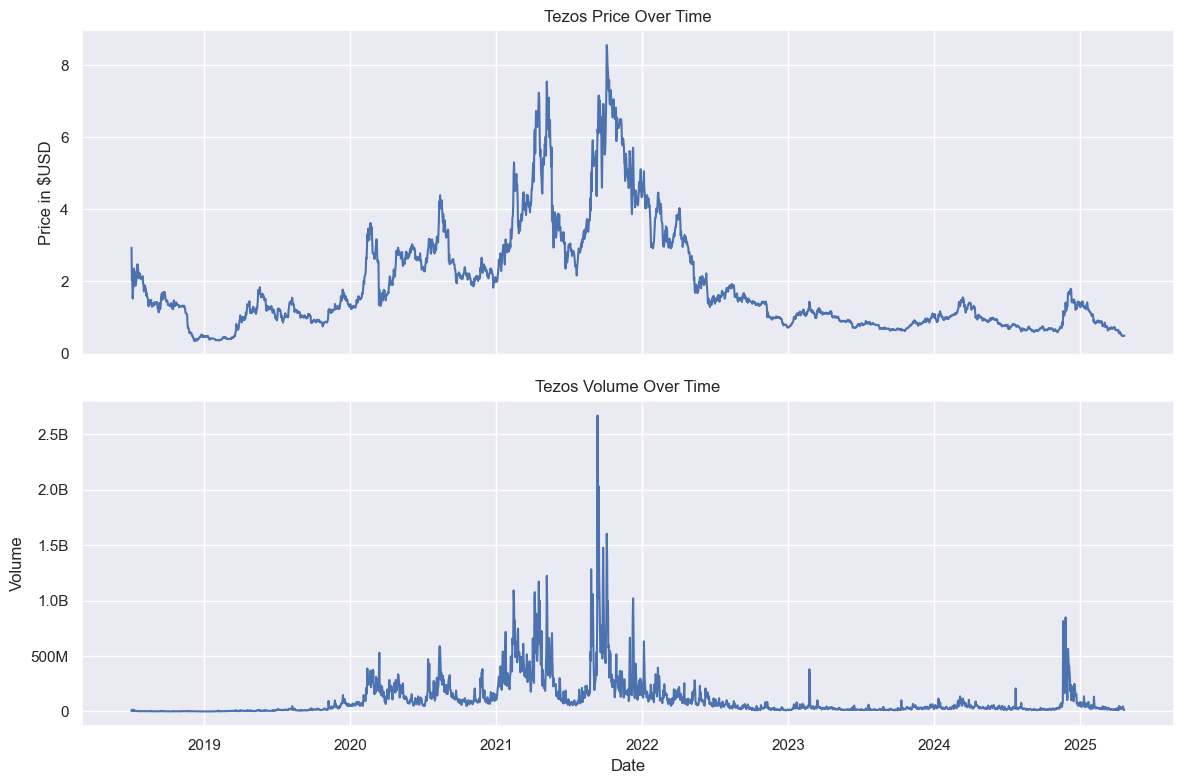
\includegraphics[width=0.8\textwidth]{Tezos_price_volume.png}
    \caption{Daily Tezos trading volume over time.}
    \label{fig:xtz-volume}
\end{figure}
The chart depicting Tezos's historical price and trading volume reveals a clear trend: both metrics generally increased until late 2021, after which they began to decline.
 Trading volume shows a particularly pronounced upward trajectory from 2018 through 2021, followed by a steady reduction to relatively low levels in recent years.
  This drop suggests a significant decrease in investor interest or market activity surrounding Tezos.
   Price movements align closely with this trend, peaking at an all-time high of \$9.12 on October 4, 2021, and subsequently declining.
    While occasional upward fluctuations have occurred—often in tandem with broader market rallies—the current price of Tezos remains considerably lower compared to its historical peak. 
    This observation underscores the diminished market enthusiasm for Tezos in the post-2021 period.

\subsubsection{Visualizing prices as a percentage of the All-Time High}
\label{sec:pricehistory-ATH}
\begin{figure}[H]
    \centering
    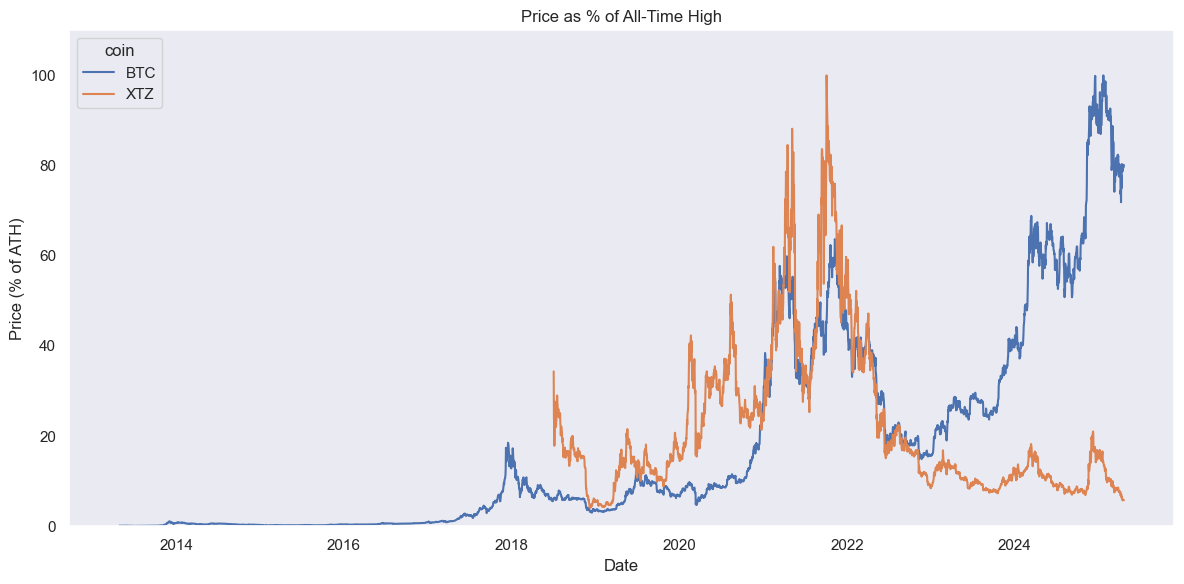
\includegraphics[width=0.8\textwidth]{athpercentage.png}
    \caption{Price of Bitcoin and Tezos as a percentage of their all-time high.}
    \label{fig:athpercentage}
\end{figure}

A common method to visualize the price history of assets is to express their prices as a percentage of their all-time high (ATH). we do this by dividing the price at each point in time by the ATH and multiplying by 100. This approach allows for a more intuitive comparison of price movements over time, regardless of the absolute price levels of the assets.
this is coded as follows:
\begin{lstlisting}[language=Python, caption={Price as a percentage of the all-time high}, label={lst:athpercentage-code}]
    dfBTC['price_pct_ath'] = dfBTC['price'] / dfBTC['price'].max() * 100
dfXTZ['price_pct_ath'] = dfXTZ['price'] / dfXTZ['price'].max() * 100
dfBTC['coin'] = 'BTC'
dfXTZ['coin'] = 'XTZ'

dfMerged = pd.concat([dfBTC,dfXTZ])

plt.figure(figsize=(12, 6))
sns.lineplot(data=dfMerged, x='date', y='price_pct_ath', hue='coin')
plt.title('Price as % of All-Time High')
plt.xlabel('Date')
plt.ylabel('Price')
plt.ylim(0, 110)
plt.tight_layout()
plt.show()
\end{lstlisting}

Figure~\ref{fig:athpercentage} presents the price trajectories of Bitcoin and Tezos expressed as a percentage of their respective all-time highs.
This normalization offers a clearer comparative perspective on the relative performance and volatility of the two assets over time. Both cryptocurrencies exhibit a broadly similar pattern, including the pronounced upward movement during the 2020–2021 bull market, followed by a period of decline.
Despite these overarching similarities, the two assets differ significantly in terms of scale and timing of price movements.
For example, there are periods in which Tezos reaches its all-time high while Bitcoin experiences only a moderate upward trend, and conversely, instances where Bitcoin achieves new record highs while Tezos displays only modest gains. These discrepancies highlight the distinct market dynamics and investor behavior influencing each asset, even within shared macroeconomic conditions.

It is also worth noting the disparity in dataset length: while Bitcoin’s historical data spans back to 2013, Tezos data begins only in mid-2018. Given that the central objective of this thesis is to predict Tezos’s price movements, the Bitcoin dataset will be truncated accordingly.

\subsubsection{Price Correlation}
\label{sec:pricecorrelation}

\begin{lstlisting}[language=Python, caption={Correlation matrix}, label={lst:correlation}]
    correlation = dfBTCfiltered['price'].corr(dfXTZfiltered['price'])
    print(correlation) #output: -0.3923556645977417
\end{lstlisting}
To examine the relationship between the daily prices of Bitcoin and Tezos, we compute the Pearson correlation coefficient.
This statistical measure quantifies the linear association between the two time series, helping to assess whether the assets tend to move together or independently. The resulting value of approximately $-0.39$ suggests a weak negative correlation, indicating that, over the examined period, the two cryptocurrencies do not consistently follow the same directional trend.

\begin{figure}[H]
    \centering
    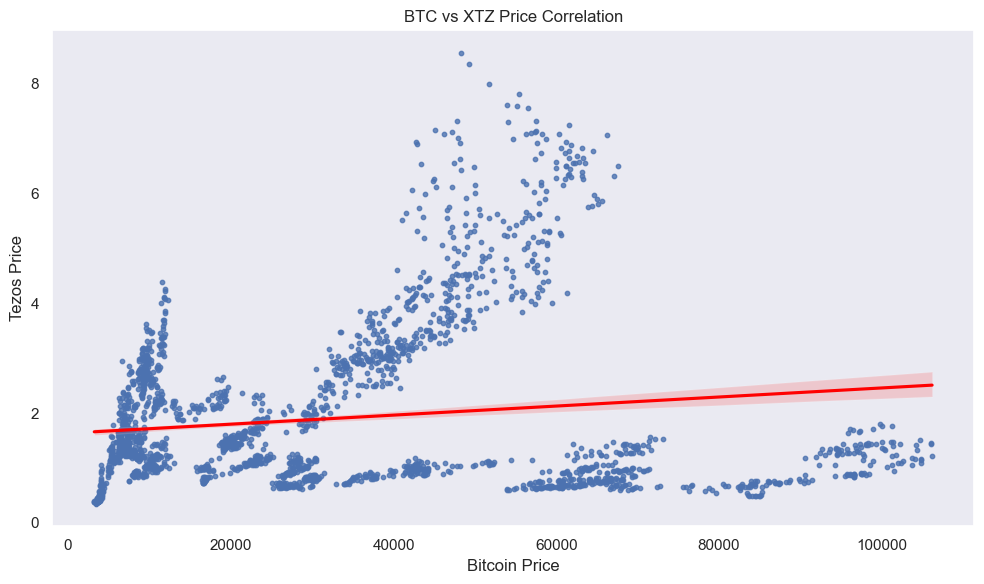
\includegraphics[width=0.85\textwidth]{scatter_price_corr.png}
    \caption{Scatter plot showing the relationship between Bitcoin and Tezos prices. A fitted regression line is included to indicate the overall trend.}
    \label{fig:price_scatter}
\end{figure}

Figure~\ref{fig:price_scatter} illustrates the relationship between the daily prices of Bitcoin and Tezos, with each point representing a single day—Bitcoin's price on the $x$-axis and Tezos's price on the $y$-axis.
 At first glance, the scatter plot appears to suggest a weak upward trend. However, the Pearson correlation coefficient of $-0.39$ indicates a moderate negative linear relationship between the two price series. 
 This apparent contradiction may be attributed to the significant difference in price scales, the clustering of data points, and potential non-linear dynamics that are not well captured by a linear trend line. 
 This emphasizes the need to supplement visual analysis with statistical measures when assessing the relationships between financial variables.